\section{Umsetzung in Code}
Im Folgenden werde ich auf die Implementierung der einzelnen Module Schritt für Schritt eingehen und die Besonderheiten, Erfahrungen und Probleme während der Programmierung beschreiben. Ich werde argumentieren, warum ich etwas auf diese Art und Weise programmiert habe und was ich mir bei der Umsetzung gedacht habe. Um die PDF Web App auch offline nutzen zu können, habe ich die Library-Dateien runtergeladen und in einem Ordner libs direkt eingebunden, anstatt \gls{cdn}-Links zu den jeweiligen Libraries zu verknüpfen. Zur Positionierung von HTML-Elementen in der PDF Web App habe ich hauptsächlich auf das CSS Flexible Box (Flex Box) Layout zurückgegriffen. 

\subsection{Werkzeuge}
\begin{itemize}
	\item Entwicklungsumgebung: Visual Studio Code
	\item ausführende Programme: Browser Firefox, Opera, Google Chrome, Microsoft Edge
	\item Sprachen: JavaScript, CSS, HTML
	\item Libraries: Vue JS 3 Version 3.0.2, PDF-LIB, pdf.js, zip,js, Bootstrap Filestyle Version 2.1.0, Bootstrap Version 4.3.1, jQuery Version 3.6.0, Alwan
	\item Tutorials: Tiddly Wiki über die Bedienung der PDF Web App
\end{itemize}

\subsection{Links der Resources}
\begin{itemize}
	\item \url{https://vuejs.org/}
	\item \url{https://pdf-lib.js.org/}
	\item \url{https://github.com/mozilla/pdf.js}
	\item \url{https://github.com/gildas-lormeau/zip.js/}
	\item \url{https://github.com/markusslima/bootstrap-filestyle}
	\item \url{https://getbootstrap.com/}
	\item \url{https://jquery.com/}
	\item \url{https://github.com/SofianChouaib/alwan}
	\item \url{https://tiddlywiki.com/}
\end{itemize}

\subsection{Ordnerstruktur}
Abbildung \ref{fig:folders} stellt die Ordnerstruktur des Projekts dar. 

\begin{figure}[!htbp]
	\centering
	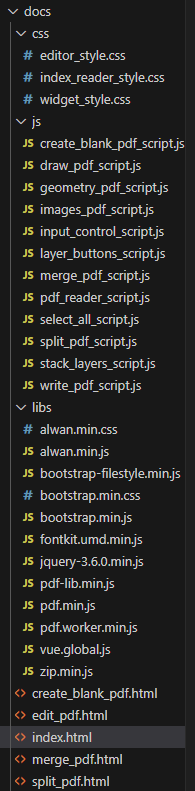
\includegraphics[width=0.3\textwidth]{"images/folders.png"}
	\caption{Ordnerstruktur der PDF Web App}
	\label{fig:folders}
\end{figure}

Im Ordner js sind meine selbst geschriebenen JavaScript-Dateien und im Ordner css meine eigenen CSS-Dateien abgelegt. Genauso wurden alle HTML-Dateien von mir erstellt. Der Ordner libs enthält alle JavaScript- und CSS-Dateien von externen Libraries. Die Datei pdf.worker.min.js ist eine dependency von pdf.js und fontkit.umd.min.js gehört zur Library PDF-LIB, um benutzerdefinierte Fonts einzubinden. Im Prinzip hat jedes Modul seine eigene JavaScript-Datei. Das Script input\_control\_script.js, welches alle Module implementiert, enthält Kontrollfunktionen für Benutzereingabefelder und die ZIP-Download-Funktionen. Der Editor enthält teilt sich die Dateien pdf\_reader\_script.js und index\_reader\_style.css mit dem Reader. Die CSS-Datei widget\_style.css deckt den Creator, Merger und Splitter ab. Der Editor besteht aus mehreren Scripten: write\_pdf\_script.js für Textelemente, draw\_pdf\_script.js für Zeichnungen, geometry\_pdf\_script.js für Shapeelemente, images\_pdf\_script.js für Bildelemente, layer\_buttons\_script.js für Ebenenmenübuttons, select\_all\_script.js für die Auswahlfilterbuttons Select All und Deselect All und stack\_layers\_script.js für Ebenenmanagementfunktionen. 


\subsection{Umsetzung der Hauptmenüführung}
Das Hauptmenü wollte ich sehr simpel und minimalistisch gestalten. Daher habe ich für die Startseite nur einen weißen Hintergrund mit einem oberen Balken in der Farbe \#333, der die Hauptmenübuttons hervorhebt. Die Buttons haben einen vordefinierten Style von der Library Bootstrap. In der Bootstrap Library kann man den Style durch bestimmte Klassen auswählen. Nicht ausgewählte Buttons haben die Bootstrap-Klasse btn-success für die grünen Buttons und der ausgewählte dunkle Button mit grüner Schrift und Umrandung hat die Bootstrap Klasse btn-outline-success. Anfangs war es schwierig den default Style des input type="file" HTML-Elements zu verändern. Vor allem die Beschriftung des Buttons für Choose file war standardmäßig in Deutsch gehalten und lies sich nicht in englischer Sprache programmieren. Daher habe ich die Library Bootstrap Filestyle verwendet, um den Choose file Button in Englisch und mit anderem Style zu versehen. Da haben sich die Bootstrap Button Styles angeboten. Um eine Designkonsistenz zu erzielen, habe ich die Bootstrap Buttons überall in der PDF Web App in verschiedenen Stylevarianten verwendet. Lediglich beim Tools Seitenmenü im Editor habe ich einen eigenen Style für die Buttons für Elementoperationen programmiert. Der Reader, Splitter und Merger bestehen aus einer separaten HTML-Seite. Das Editormodul ist eine einzelne HTML-Seite, bei der je nach Funktion die entsprechenden Schaltflächen für die Elementoperationen mit display: flex eingeblendet und mit display: none ausgeblendet werden. 


\subsection{Implementierung des Reader Moduls}
Die Basisstruktur der Funktion für den Choose file Button ist im folgenden Codeabschnitt dargestellt:

\begin{lstlisting}[caption=Einlesen einer PDF-Datei]
	inputFileButtons[i].addEventListener("change", function(e) {
		file = e.target.files[0];
		const fileReader = new FileReader(); 
		fileReader.onload = function() {
			const typedarray = new Uint8Array(this.result);
			pdfState.originalPDFBytes = typedarray;
			const loadingTask = pdfjsLib.getDocument(typedarray);
			loadingTask.promise.then(async (pdf) => {
				pdfState.pdf = pdf;
			});
		}
		if (file) {
			fileReader.readAsArrayBuffer(file);
		}
	}, false);
\end{lstlisting} 

Das Objekt für das eingelesene PDF ist wie folgt strukturiert:

\begin{lstlisting}[caption=PDF-Datei Objekt]
	let pdfState = {
		pdf: null,
		currentPage: 1,
		lastPage: 1,
		renderedPage: 0,
		zoom: 1,
		originalPDFBytes: null,
		existingPDFBytes: null,
		originalWidths: [],
		originalHeights: []
	}
\end{lstlisting} 